\section{Le module \touistplan}
\fred{Exemple PDDL (verbatim) + codage \touist + sortie SAT, QBF, SMT}

\subsection{Le langage PDDL (Planning Domain Definition Language)}

Le langage PDDL~\fred{citer McDermott98} permet d'une part de définir des domaines de planification, c'est à dire une modélisation d'ensembles d'actions, et d'autre part des problèmes de planification relatifs à un domaine particulier, c'est à dire un état initial et un but qui devra être satisfait après avoir exécuté un plan d'actions choisies parmi les actions du domaine.

\paragraph*{Un exemple, le domaine Gripper :} Robby doit transporter des balles entre différentes salles. Les capacités du robot sont de pouvoir prendre une balle dans l'une de ses pinces, déposer une balle ou se déplacer d'une salle à une autre.%\\

\begin{center}
  \begin{minipage}[c]{.38\linewidth}
   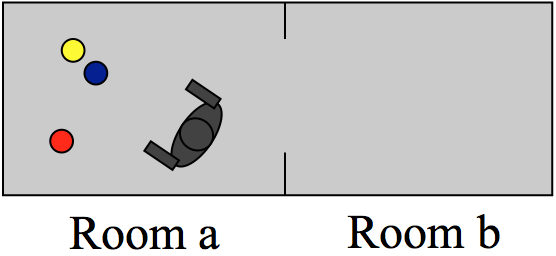
\includegraphics[scale=0.55]{figures/robby_a_3balls.png}
  \end{minipage}
  \begin{minipage}[c]{.05\linewidth}
    $\Rightarrow$
  \end{minipage}
  \begin{minipage}[c]{.38\linewidth}
    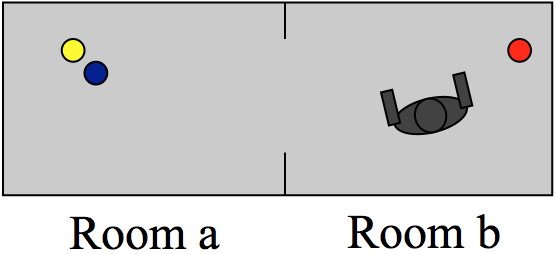
\includegraphics[scale=0.55]{figures/robby_b_3balls.png}
  \end{minipage}
\end{center}

\newpage

\noindent Les fluents (non instanciés) de ce domaine peuvent être défini par :
%$F=\{at-robby(x),at(x,y),free(x),carry(x,y)\}$\\
%\noindent La sémantique de ces fluents est la suivante :
\begin{itemize}
	\item $at$-$robby(x)$: Robby est dans la salle $x$ ;
	\item $at(x,y)$: La balle $x$ est dans la salle $y$ ;
	\item $free(x)$: La pince $x$ est libre ;
	\item $carry(x,y)$: Robby transporte la balle $x$ dans sa pince $y$.
\end{itemize}

\noindent L'ensemble des opérateurs (actions non instanciées) de ce domaine peut être défini par :\\ $O=\{MOVE(x,y),PICK(x,y,z),DROP(x,y,z)\}$\\

\noindent $Prec(MOVE(x,y)) = \{at$-$robby(x)\}$\\
$Add(MOVE(x,y)) = \{at$-$robby(y)\}$\\
$Del(MOVE(x,y)) = \{at$-$robby(x)\}$\\

\noindent $Prec(PICK(x,y,z)) = \{at(x,y),at$-$robby(y),free(z)\}$\\
$Add(PICK(x,y,z)) = \{carry(x,z)\}$\\
$Del(PICK(x,y,z)) = \{at(x,y),free(z)\}$




\paragraph{Définition du domaine en PDDL :}~\\
\fbox{
\begin{minipage}[c]{\linewidth}
\lstset{escapeinside={<@}{@>}}
\lstset{language=pddl}
\begin{lstlisting}
(define (domain gripper-strips)
    (:requirements :strips :typing)
    (:types room gripper ball)
    (:predicates (at-robby ?r - room)
        (at ?b - ball ?r - room)
        (free ?g - gripper)
        (carry ?b - ball ?g - gripper))
...<@\fbox{Définition des actions}@>...)
\end{lstlisting}
\end{minipage}
}

%\begin{scriptsize}
\begin{center}
\fbox{
\texttt{
\begin{minipage}[c]{\linewidth}
\begin{tabbing}
(\bb{define} (\bb{domain} gripper-strips) \hspace{-6cm} \= \hspace{2.3cm} \= \hspace{3.2cm} \\
\>  (\bb{:requirements :strips :typing})\\
\>  (\bb{:types} room gripper ball)\\
\>   (\bb{:predicates} (at-robby ?r - room)\\
\> \>		(at ?b - ball ?r - room)\\
\> \>		(free ?g - gripper)\\
\> \>		(carry ?b - ball ?g - gripper))\\
\\
$\cdots$ \fbox{Définition des actions} $\cdots$)
\end{tabbing}
\end{minipage}
}}
\end{center}
%\end{scriptsize}


\paragraph{Définition des actions en PDDL :}~\\

%\fbox{\texttt{
%\begin{minipage}[c]{\linewidth}
%\begin{tabbing}
%(:action move \hspace{-2cm} \= \hspace{1.5cm} \= \\
%\>     :parameters  (?from ?to) \\
%\>     :precondition (and  (room ?from) (room ?to) (at-robby ?from))\\
%\>     :effect (and  (at-robby ?to)\\
%\>	\>	     (not (at-robby ?from))))
%\end{tabbing}
%\end{minipage}
%}}

\begin{center}
\fbox{\texttt{
\begin{minipage}[c]{\linewidth}
\begin{tabbing}
(\bb{:action} move \hspace{-2cm} \= \hspace{1.5cm} \= \\
\>     \bb{:parameters}  (?from - room ?to - room) \\
\>     \bb{:precondition} (at-robby ?from)\\
\>     \bb{:effect} (and  (at-robby ?to)\\
\>	\>	     (not (at-robby ?from))))
\end{tabbing}
\end{minipage}
}}
\end{center}

\begin{center}
\fbox{\texttt{
\begin{minipage}[c]{\linewidth}
\begin{tabbing} 
(\bb{:action} pick \hspace{-2cm} \= \hspace{3.5cm} \= \\
\>       \bb{:parameters} (?b - ball ?r - room ?g - gripper)\\
\>       \bb{:precondition}  (and (at ?b ?r)\\
\> \> (at-robby ?r)\\
\> \> (free ?g))\\
\>       \bb{:effect} (and (carry ?b ?g)\\
\> \>		    (not (at ?b ?r)) \\
\> \>		    (not (free ?g))))\\
\end{tabbing}
\end{minipage}
}}
\end{center}

L'action \texttt{pick} permet au robot de prendre dans une salle un balle avec l'une de ses pinces.

\begin{center}
\fbox{\texttt{
\begin{minipage}[c]{\linewidth}
\begin{tabbing} 
(\bb{:action} drop \hspace{-2cm} \= \hspace{3.5cm} \= \\
\>       \bb{:parameters} (?b - ball ?r - room ?g - gripper)\\
\>       \bb{:precondition}  (and (carry ?b ?g)\\
\> \> (at-robby ?r)\\
\>       \bb{:effect} (and (at ?b ?r)\\
\> \>		    (not (carry ?b ?g)) \\
\> \>		    (free ?g)))\\
\end{tabbing}
\end{minipage}
}}
\end{center}

L'action \texttt{drop} permet au robot de déposer dans une salle un balle qu'il tient dans l'une de ses pinces.


\paragraph{Définition d'un problème en PDDL :}~\\

\begin{center}
\fbox{\texttt{
\begin{minipage}[c]{\linewidth}
\begin{tabbing}
(\bb{define} (\bb{problem} gripper-2) \hspace{-5cm} \= \hspace{0.5cm} \= \hspace{4cm} \\
\> (\bb{:domain} gripper-strips)\\
\> (\bb{:objects}\\
\> \> rooma roomb - room\\
\> \> left right - gripper\\
\> \> ball1 ball2 - ball)\\
\> (\bb{:init}\\
\> \> (free left) (free right)\\
\> \> (at ball1 rooma) (at ball2 rooma)\\
\> \> (at-robby rooma))\\
\> (\bb{:goal}\\
\> \> (and (at ball1 roomb) (at ball2 roomb))))
\end{tabbing}
\end{minipage}
}}
\end{center}


\subsection{Extraction d'un plan avec le module \touistplan}

%\subsubsection{Codage SAT dans les espaces d'états avec frame-axiomes explicatifs pour le problème Gripper-3}

%\begin{scriptsize}
%\begin{verbatim}
%Select TouIST 3.5.2
%Select [LANGUAGE] EncodingRules: [SAT] Explanatory Frame-axioms
%Select SAT SOLVER: Glucose
%
%Searching solution with SATPLAN (Explanatory Frame-Axioms)...
%
%Maximum plan length: 2^|Fluents|=256.
%Searching solution with length 1...
%--- TouIST solve (SAT) / length = 1 ---
%Searching solution with length 2...
%--- TouIST solve (SAT) / length = 2 ---
%Searching solution with length 3...
%--- TouIST solve (SAT) / length = 3 ---
%Searching solution with length 4...
%--- TouIST solve (SAT) / length = 4 ---
%Searching solution with length 5...
%--- TouIST solve (SAT) / length = 5 ---
%Searching solution with length 6...
%--- TouIST solve (SAT) / length = 6 ---
%Searching solution with length 7...
%--- TouIST solve (SAT) / length = 7 ---
%Solution found at length 7.
%1 A_PICK_ball1_rooma_left(1)
%1 A_PICK_ball3_rooma_right(1)
%1 A_MOVE_rooma_roomb(2)
%1 A_DROP_ball3_roomb_right(3)
%1 A_MOVE_roomb_rooma(4)
%1 A_PICK_ball2_rooma_right(5)
%1 A_MOVE_rooma_roomb(6)
%1 A_DROP_ball2_roomb_right(7)
%1 A_DROP_ball1_roomb_left(7)
%\end{verbatim}
%\end{scriptsize}

%\begin{figure}[h]\label{gripper3:sat-efa}
%\begin{footnotesize}
%  \xymatrix@C=0.1pc@R=1pc{
%  \text{S}_{0} (\textit{Init}) \ar@{>}[r] & \fbox{\substack{\gripperpick{1}{a}{left}\\\gripperpick{3}{a}{right}}} \ar@{>}[r]  & \fbox{\substack{\grippermove{a}{b}}} \ar@{>}[r] & \fbox{\substack{\gripperdrop{3}{b}{right}}} \ar@{>}[r] & \fbox{\substack{\grippermove{b}{a}}}
%  \ar@{>}[r] & \fbox{\substack{\gripperpick{2}{a}{right}}} \ar@{>}[r] & \fbox{\substack{\grippermove{a}{b}}} \ar@{>}[r] & \fbox{\substack{\gripperdrop{2}{b}{right}\\\gripperdrop{1}{b}{left}}} \ar@{>}[r] & \text{S}_{8} (\textit{Goal}) \\
%  }
% \end{footnotesize}
%\caption{Transitions du plan en 7 étapes retourné par \touistplan pour le problème Gripper-3 (codage SAT de longueur 7 dans les espaces d'états avec frame-axiomes explicatifs)}
%\end{figure}


%\subsubsection{Codage d'arbre compact QBF dans les espaces d'états avec frame-axiomes explicatifs pour le problème Gripper-3}

%\begin{scriptsize}
%\begin{verbatim}
%Select TouIST 3.5.2
%Select [LANGUAGE] EncodingRules: [QBF] Explanatory Frame-axioms
%Select QBF SOLVER: RAReQS
%
%Searching solution with QBFPLAN (Explanatory Frame-Axioms)...
%
%Maximum tree depth: |Fluents|=16.
%Searching solution at depth 1...
%--- TouIST solve (QBF) / branch atom =  ---
%Searching solution at depth 2...
%--- TouIST solve (QBF) / branch atom =  ---
%Plan existence time (PLANSAT): 0.14
%Solution found at depth 2.
%and A_MOVE_roomb_rooma(2)
%--- TouIST solve (QBF) / branch atom = and not b(2) ---
%and A_MOVE_rooma_roomb(1)
%--- TouIST solve (QBF) / branch atom = and not b(1) ---
%and A_PICK_ball1_rooma_left(0)
%and A_PICK_ball3_rooma_right(0)
%--- TouIST solve (QBF) / branch atom = and b(1) ---
%and A_DROP_ball3_roomb_right(0)
%--- TouIST solve (QBF) / branch atom = and b(2) ---
%and A_MOVE_rooma_roomb(1)
%--- TouIST solve (QBF) / branch atom = and not b(1) ---
%and A_PICK_ball2_rooma_right(0)
%--- TouIST solve (QBF) / branch atom = and b(1) ---
%and A_DROP_ball1_roomb_left(0)
%and A_DROP_ball2_roomb_right(0)
%Plan existence time (PLANSAT): 0.14
%Plan extract time: 0.54
%\end{verbatim}
%\end{scriptsize}

%\begin{figure}[h]\label{gripper3:qbf-efa}
%\begin{footnotesize}
%   %\hspace{0.8em}
%   \xymatrix@C=-3.6pc@R=3pc{
%   & & & & & *+[F]+{\substack{\grippermove{b}{a}}} %\ar@{.}[lld]_{b_{2}=\bot} \ar@{.}[rrd]^{b_{2}=\top} \ar@/^1pc/[rdd] & & & & \\
%   & & & *+[F]+{\substack{\grippermove{a}{b}}} \ar[rd]^{b_{1}=\top} & & & & *+[F]+{\substack{\grippermove{a}{b}}} \ar[rd]^{b_{1}=\top} & & \\
%    & & *+[F]+{\substack{\gripperpick{1}{a}{left} \\ \gripperpick{3}{a}{right}}} \ar[ru]^{b_{1}=\bot}  & & *+[F]+{\substack{\gripperdrop{3}{b}{right}}} \ar@/^1pc/[ruu] & &  *+[F]+{\substack{\gripperpick{2}{a}{right}}} \ar[ru]^{b_{1}=\bot} & & *+[F]+{\substack{\gripperdrop{1}{b}{left}\\\gripperdrop{2}{b}{right}}} \\
%  }
% \end{footnotesize}
%\caption{Transitions du plan en 7 étapes retourné par \touistplan pour le problème Gripper-3 (codage d'arbre compact QBF (CTE) de profondeur 2 dans les espaces d'états avec frame-axiomes explicatifs}
%\end{figure}


\subsubsection{Codage SAT dans les espaces d'états avec frame-axiomes explicatifs pour le problème Gripper-7}

\begin{scriptsize}
\begin{verbatim}
Select TouIST 3.5.2
Select [LANGUAGE] EncodingRules: [SAT] Explanatory Frame-axioms
Select SAT SOLVER: Glucose

Searching solution with SATPLAN (Explanatory Frame-Axioms)...

Maximum plan length: 2^|Fluents|=256.
Searching solution with length 1...
--- TouIST solve (SAT) / length = 1 ---
Searching solution with length 2...
--- TouIST solve (SAT) / length = 2 ---
Searching solution with length 3...
--- TouIST solve (SAT) / length = 3 ---
Searching solution with length 4...
--- TouIST solve (SAT) / length = 4 ---
Searching solution with length 5...
--- TouIST solve (SAT) / length = 5 ---
Searching solution with length 6...
--- TouIST solve (SAT) / length = 6 ---
Searching solution with length 7...
--- TouIST solve (SAT) / length = 7 ---
Searching solution with length 8...
--- TouIST solve (SAT) / length = 8 ---
Searching solution with length 9...
--- TouIST solve (SAT) / length = 9 ---
Searching solution with length 10...
--- TouIST solve (SAT) / length = 10 ---
Searching solution with length 11...
--- TouIST solve (SAT) / length = 11 ---
Searching solution with length 12...
--- TouIST solve (SAT) / length = 12 ---
Searching solution with length 13...
--- TouIST solve (SAT) / length = 13 ---
Searching solution with length 14...
--- TouIST solve (SAT) / length = 14 ---
Searching solution with length 15...
--- TouIST solve (SAT) / length = 15 ---
Solution found at length 15.
1 A_PICK_ball2_rooma_left(1)
1 A_PICK_ball3_rooma_right(1)
1 A_MOVE_rooma_roomb(2)
1 A_DROP_ball3_roomb_right(3)
1 A_DROP_ball2_roomb_left(3)
1 A_MOVE_roomb_rooma(4)
1 A_PICK_ball7_rooma_left(5)
1 A_PICK_ball6_rooma_right(5)
1 A_MOVE_rooma_roomb(6)
1 A_DROP_ball6_roomb_right(7)
1 A_DROP_ball7_roomb_left(7)
1 A_MOVE_roomb_rooma(8)
1 A_PICK_ball1_rooma_right(9)
1 A_PICK_ball5_rooma_left(9)
1 A_MOVE_rooma_roomb(10)
1 A_DROP_ball5_roomb_left(11)
1 A_MOVE_roomb_rooma(12)
1 A_PICK_ball4_rooma_left(13)
1 A_MOVE_rooma_roomb(14)
1 A_DROP_ball1_roomb_right(15)
1 A_DROP_ball4_roomb_left(15)
\end{verbatim}
\end{scriptsize}

\begin{figure}[h]\label{gripper7:sat-efa}
\begin{footnotesize}
  \xymatrix@C=-6.1pc@R=0.5pc{
   *+[F]+{\substack{\gripperpick{2}{a}{left}\\\gripperpick{3}{a}{right}}} \ar@{>}[rd] \\
  & *+[F]+{\substack{\grippermove{a}{b}}} \ar@{>}[rd] \\
  & & *+[F]+{\substack{\gripperdrop{3}{b}{right}\\\gripperdrop{2}{b}{left}}} \ar@{>}[rd] \\
  & & & *+[F]+{\substack{\grippermove{b}{a}}}
  \ar@{>}[rd] \\
  & & & & *+[F]+{\substack{\gripperpick{7}{a}{left}\\\gripperpick{6}{a}{right}}} \ar@{>}[rd] \\
  & & & & & *+[F]+{\substack{\grippermove{a}{b}}} \ar@{>}[rd] \\
  & & & & & & *+[F]+{\substack{\gripperdrop{6}{b}{right}\\\gripperdrop{7}{b}{left}}} \ar@{>}[rd] \\
  & & & & & & & *+[F]+{\substack{\grippermove{b}{a}}} \ar@{>}[rd] \\
  & & & & & & & & *+[F]+{\substack{\gripperpick{1}{a}{right}\\\gripperpick{5}{a}{left}}} \ar@{>}[rd] \\
  & & & & & & & & & *+[F]+{\substack{\grippermove{a}{b}}} \ar@{>}[rd] \\
  & & & & & & & & & & *+[F]+{\substack{\gripperdrop{5}{b}{left}}} \ar@{>}[rd] \\
  & & & & & & & & & & & *+[F]+{\substack{\grippermove{b}{a}}} \ar@{>}[rd] \\
  & & & & & & & & & & & & *+[F]+{\substack{\gripperpick{4}{a}{left}}} \ar@{>}[rd] \\
  & & & & & & & & & & & & & *+[F]+{\substack{\grippermove{a}{b}}} \ar@{>}[rd] \\
  & & & & & & & & & & & & & & *+[F]+{\substack{\gripperdrop{1}{b}{right}\\\gripperdrop{4}{b}{left}}}
  }
 \end{footnotesize}
\caption{Représentation linéaire du plan en 15 étapes retourné par \touistplan pour le problème Gripper-7 (codage SAT de longueur 15 dans les espaces d'états avec frame-axiomes explicatifs)}
\end{figure}

\subsubsection{Codage d'arbre compact QBF dans les espaces d'états avec frame-axiomes explicatifs pour le problème Gripper-7}

\begin{scriptsize}
\begin{verbatim}
Select TouIST 3.5.2
Select [LANGUAGE] EncodingRules: [QBF] Explanatory Frame-axioms
Select QBF SOLVER: RAReQS

Searching solution with QBFPLAN (Explanatory Frame-Axioms)...

Maximum tree depth: |Fluents|=32.
Searching solution at depth 1...
--- TouIST solve (QBF) / branch atom =  ---
Searching solution at depth 2...
--- TouIST solve (QBF) / branch atom =  ---
Searching solution at depth 3...
--- TouIST solve (QBF) / branch atom =  ---
Plan existence time (PLANSAT): 1.41
Solution found at depth 3.
and A_MOVE_roomb_rooma(3)
--- TouIST solve (QBF) / branch atom = and not b(3) ---
and A_MOVE_roomb_rooma(2)
--- TouIST solve (QBF) / branch atom = and not b(2) ---
and A_MOVE_rooma_roomb(1)
--- TouIST solve (QBF) / branch atom = and not b(1) ---
and A_PICK_ball4_rooma_left(0)
and A_PICK_ball3_rooma_right(0)
--- TouIST solve (QBF) / branch atom = and b(1) ---
and A_DROP_ball4_roomb_left(0)
and A_DROP_ball3_roomb_right(0)
--- TouIST solve (QBF) / branch atom = and b(2) ---
and A_MOVE_rooma_roomb(1)
--- TouIST solve (QBF) / branch atom = and not b(1) ---
and A_PICK_ball2_rooma_right(0)
and A_PICK_ball1_rooma_left(0)
--- TouIST solve (QBF) / branch atom = and b(1) ---
and A_DROP_ball2_roomb_right(0)
and A_DROP_ball1_roomb_left(0)
--- TouIST solve (QBF) / branch atom = and b(3) ---
and A_MOVE_roomb_rooma(2)
--- TouIST solve (QBF) / branch atom = and not b(2) ---
and A_MOVE_rooma_roomb(1)
--- TouIST solve (QBF) / branch atom = and not b(1) ---
and A_PICK_ball7_rooma_right(0)
and A_PICK_ball6_rooma_left(0)
--- TouIST solve (QBF) / branch atom = and b(1) ---
and A_DROP_ball6_roomb_left(0)
and A_DROP_ball7_roomb_right(0)
--- TouIST solve (QBF) / branch atom = and b(2) ---
and A_MOVE_rooma_roomb(1)
--- TouIST solve (QBF) / branch atom = and not b(1) ---
and A_PICK_ball5_rooma_left(0)
--- TouIST solve (QBF) / branch atom = and b(1) ---
and A_DROP_ball5_roomb_left(0)
\end{verbatim}
\end{scriptsize}

\begin{figure}[h]\label{gripper7:qbf-efa}
\begin{scriptsize}
   %\hspace{0.8em}
   \xymatrix@C=-3.2pc@R=3pc{
   & & & & & & & & & *+[F]+{\substack{\grippermove{b}{a}}} \ar@{.}[lllld]_{b_{3}=\bot}\\
   & & & & & *+[F]+{\substack{\grippermove{b}{a}}} \ar@{.}[lld]_{b_{2}=\bot} \ar@{.}[rrd]^{b_{2}=\top} \ar@/^1pc/[rdd] & & & & \\
   & & & *+[F]+{\substack{\grippermove{a}{b}}} \ar[rd]^{b_{1}=\top} & & & & *+[F]+{\substack{\grippermove{a}{b}}} \ar[rd]^{b_{1}=\top} & & \\
    & & *+[F]+{\substack{\gripperpick{4}{a}{left} \\ \gripperpick{3}{a}{right}}} \ar[ru]^{b_{1}=\bot}  & & *+[F]+{\substack{\gripperdrop{4}{b}{left} \\ \gripperdrop{3}{b}{right}}} \ar@/^1pc/[ruu] & &  *+[F]+{\substack{\gripperpick{2}{a}{right} \\ \gripperpick{1}{a}{left}}} \ar[ru]^{b_{1}=\bot} & & *+[F]+{\substack{\gripperdrop{2}{b}{right}\\\gripperdrop{1}{b}{left}}} \ar@/^1pc/[ruuu] \\
  } \vspace{1em}
   %\hspace{0.8em}
   \xymatrix@C=-3.2pc@R=3pc{
   & *+[F]+{\substack{\grippermove{b}{a}}} \ar@{.}[rrrrd]^{b_{3}=\top} \ar@/^1pc/[rddd] & & & & & & & & \\
   & & & & & *+[F]+{\substack{\grippermove{b}{a}}} \ar@{.}[lld]_{b_{2}=\bot} \ar@{.}[rrd]^{b_{2}=\top} \ar@/^1pc/[rdd] & & & & \\
   & & & *+[F]+{\substack{\grippermove{a}{b}}} \ar[rd]^{b_{1}=\top} & & & & *+[F]+{\substack{\grippermove{a}{b}}} \ar[rd]^{b_{1}=\top} & & \\
    & & *+[F]+{\substack{\gripperpick{7}{a}{right} \\ \gripperpick{6}{a}{left}}} \ar[ru]^{b_{1}=\bot}  & & *+[F]+{\substack{\gripperdrop{6}{b}{left}\\\gripperdrop{7}{b}{right}}} \ar@/^1pc/[ruu] & &  *+[F]+{\substack{\gripperpick{5}{a}{left}}} \ar[ru]^{b_{1}=\bot} & & *+[F]+{\substack{\gripperdrop{5}{b}{left}}} \\
  }
 \end{scriptsize}
\caption{Représentation de l'arbre compact développé (sous-arbre gauche pour $b_{3}=\bot$ et sous-arbre droit pour $b_{3}=\top$) permettant d'extraire le plan en 15 étapes retourné par \touistplan pour le problème Gripper-7 (codage d'arbre compact QBF (CTE) de profondeur 3 dans les espaces d'états avec frame-axiomes explicatifs).}
\end{figure}